in der messung in davos \ref{}

In dem Bild \ref{img:Varianz} wurde Schnee in einem 0.2 m^2 Fläche gemessen. Ziel war es die Varianz von vergleichbarem Schnee zu ermittelt.

mit ishiwaw \ref{} wurde das Problem der hohen varianz genauer analysiert.


\begin{figure}
    \centering
    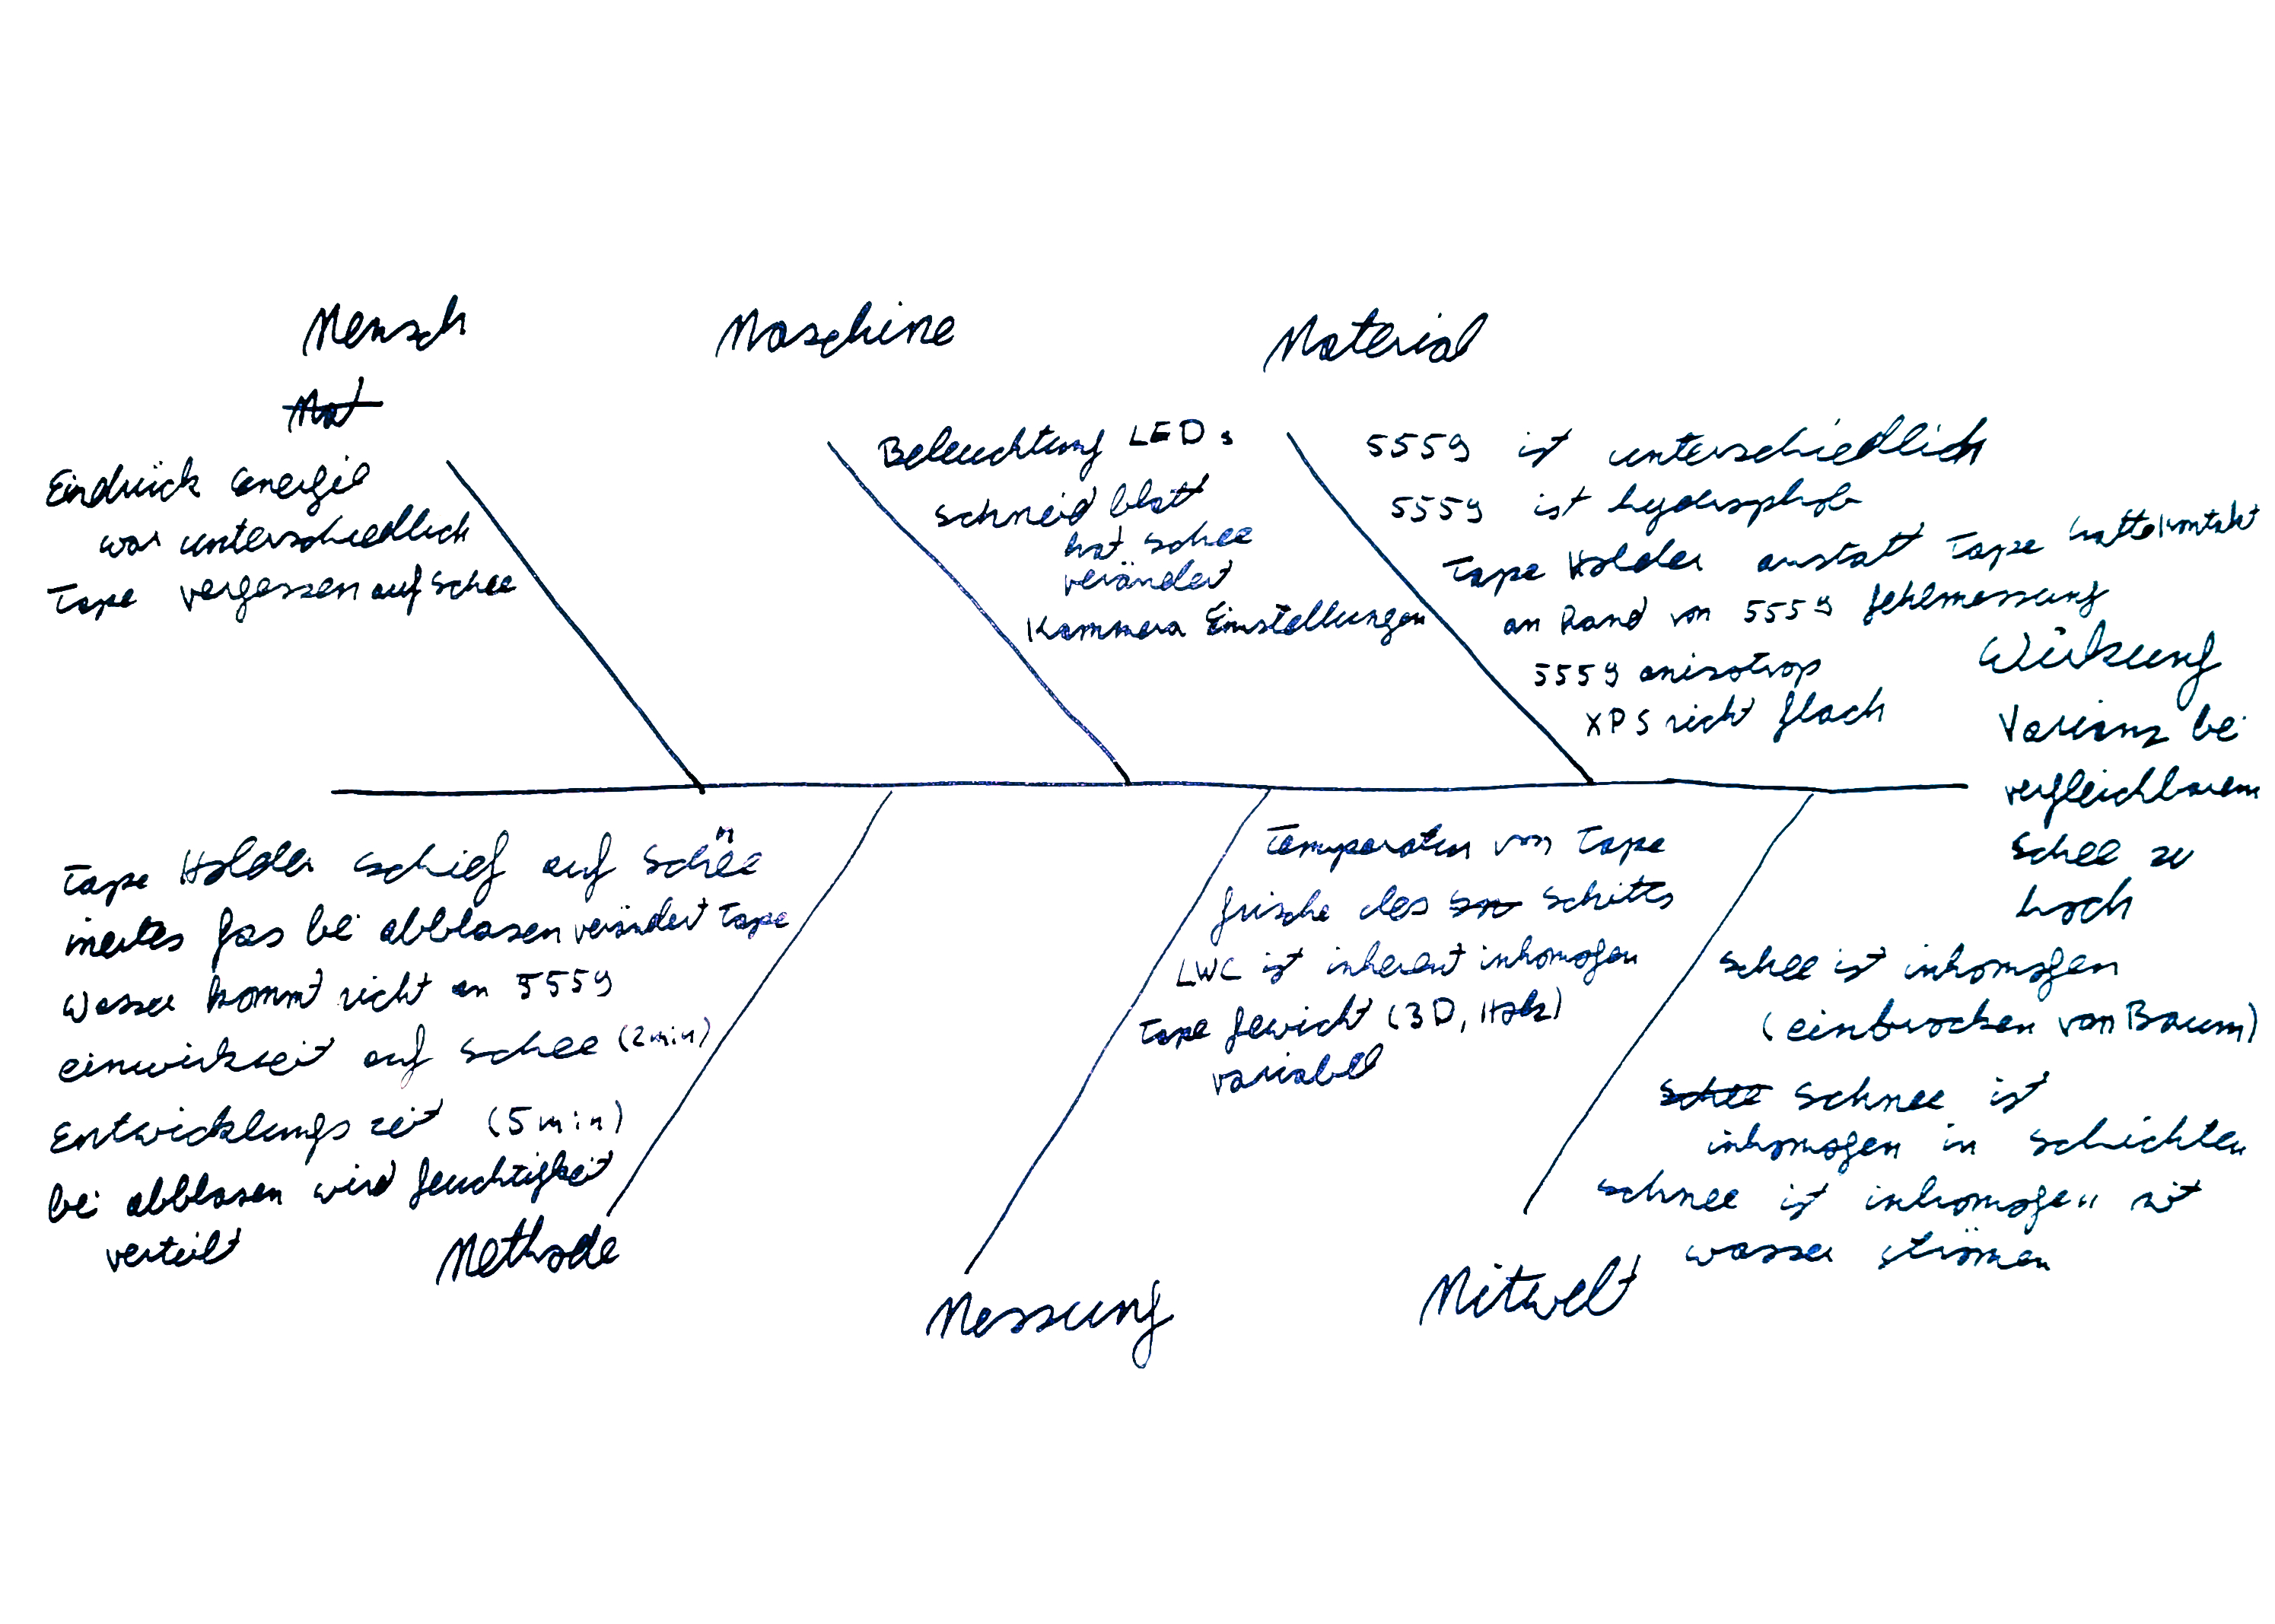
\includegraphics[width=0.8\textwidth]{Bilder/IshikawaDavos.jpg}
    \caption{Ishikawa Fehler Analyse für die Messung des Funktionsmusters 2}
    \label{fig:IshikwaDavos}
\end{figure}



die wichtigsten Einflüsse sind
\begin{itemize}
\item das Tap ist anisotrop, durch die Herstellung. das ist besonders auffällig an den Rändern. die Lösung wurde in \ref{fig:Bildverarbeitnugskonzpet} schon intuitiv benutzt. Der Rand (etwa 2 mm) soll nicht beachtet werden. der bildausschnitt wird in Zukunft so gewählt, dass der Rand nicht im Bild ist.
\item das tap hat einen schlechten kontakt zum wasser auf dem schnee. um diese hypothese zu überprüfen wurde der Winkel eines wassertropfens auf dem tape gemessen. mit einem winkel von 90 grad ist das tap genau zwischen hydrophob und hydrophil.
\item die beleuchtung war nicht homogen. deswegen werden zeit LEDs mit difusoren in dem nächsten \ref{} funktionsmuster verbaut.
\item die tape holder standen nicht genau senkrecht. deswegen wurde die führung mit den magnet bögen und stativmaterial gebaut.
\item die eindrückenergie war inkostistent. deswegen wurden die haupzahl der versuche ohne extra energie durchgeführt. bei dem durchgang mit enerigie wurde das stativmaterial benutzt um eine gleiche Potentiolle energie sicher zu stellen.
\item der tapeholder und nicht das tape hatten kontakt zum schnee. deswegen wurde der neue tapeholder umkonstruiert sodass 40 mm nur der XPS schaumstoff mit dem tape in den schnee eindringen kann.
\item der XPS schaumstoff ist nicht flach. deswegen wurde eine schneidlehre gebaut um den XPS senkrecht  zu schneiden. weiter möglichkeiten wären eine Glassplatte (mikroskop objektivtrager) zwischen den XPS und das Tape zu machen. Oder ein plastisch verformbaren träger für das tape zu entwickeln.
\item die temperatur des tapes war vor dem schneekontakt die umgebungstemeperatur (viel). deswegen wurde jedes tape runtergekülht und mit der wärembildkamera überprüft.
\item die gewichte der tape holders war um rund 10 \% unterschiedlich, denn es wurden verschiedene Versionen benutzt. die neue hat nur eine einzieg version an tape holders.
\item der schnee ist inhomogen. die messung war unter einem baum, von dem schnee und eis runter gefallet war. das hat dazu geführt, dass im schnee centimeter grosse einregionen waren.
\item der schnee ist inhomogen in schichten. im den nächsten messunng wurde ein weniger geschichteter schnee gewählt.
\item der schnee ist inhomogen mit wasser störmen. die messung in davos war in der nähe eines Baches. die nächste messung wurde ein homogener schnee gewählt.
\item die ebende auf der das tape geklebt ist, ist nicht eben, sondern beim transpornt eingedrückt worden. um das problem zu reduzieren wurden Pelican Boxen für den Transport benutzt.
\end{itemize}

weiter mögliche gründe und die sturktiurung der Gründe können im Ishikawa Diadram gesehen werden. \ref{img:ishikawa}
